\documentclass{article}
\usepackage[utf8]{inputenc}
\usepackage{amsmath, amsfonts, amssymb, amsthm}
\usepackage{graphicx}
\usepackage{geometry}
\usepackage{xcolor}

\newcommand{\inv}{^{-1}}   
\newcommand{\Z}{\mathbb Z}
\newcommand{\R}{\mathbb R}
\newcommand{\Q}{\mathbb Q}
\newcommand{\C}{\mathbb C}
\newcommand{\N}{\mathbb N}
\newcommand{\B}{\mathcal B}

\date{Due Friday, February 26, 2021}
\author{Ben Kallus}
\title{Topology \\ Homework 3}

\begin{document}
\pagecolor{black}
\color{white}
\maketitle

\noindent{\bf 1.}
\begin{proof}
    Let $\tau_X$, $\tau_Y$ be topologies on $X$ and $Y$.
    Let $\tau$ be the product topology on $X \times Y$.
    Let $C \in \tau$.
    Then, by Lemma 13.1, there exists $\mathcal D \subseteq \B$ such that $C = \bigcup\limits_{D \in \mathcal D} D$.
    Then,
    \begin{align*}
    \pi_1(C) &= \pi_1\left(\bigcup\limits_{D \in \mathcal D} \pi_1(D) \times \pi_2(D) \right) \\
    &= \bigcup\limits_{D \in \mathcal D} \pi_1(D).
    \end{align*}
    By the definition of the order topology on $X \times Y$, $\pi_1(D) \in \tau_X$ for all $D \in \mathcal D$.
    Thus, $\pi_1(C) \in \tau_X$.
    By a symmetric argument, $\pi_2(C) \in \tau_Y$.
    Thus, $\pi_1$ and $\pi_2$ map open sets to open sets.
\end{proof}

\newpage\noindent{\bf 2.}
\begin{center}
$\R^2:$

(Imagine that the whole plane is shaded, if you'd rather.)
\medskip
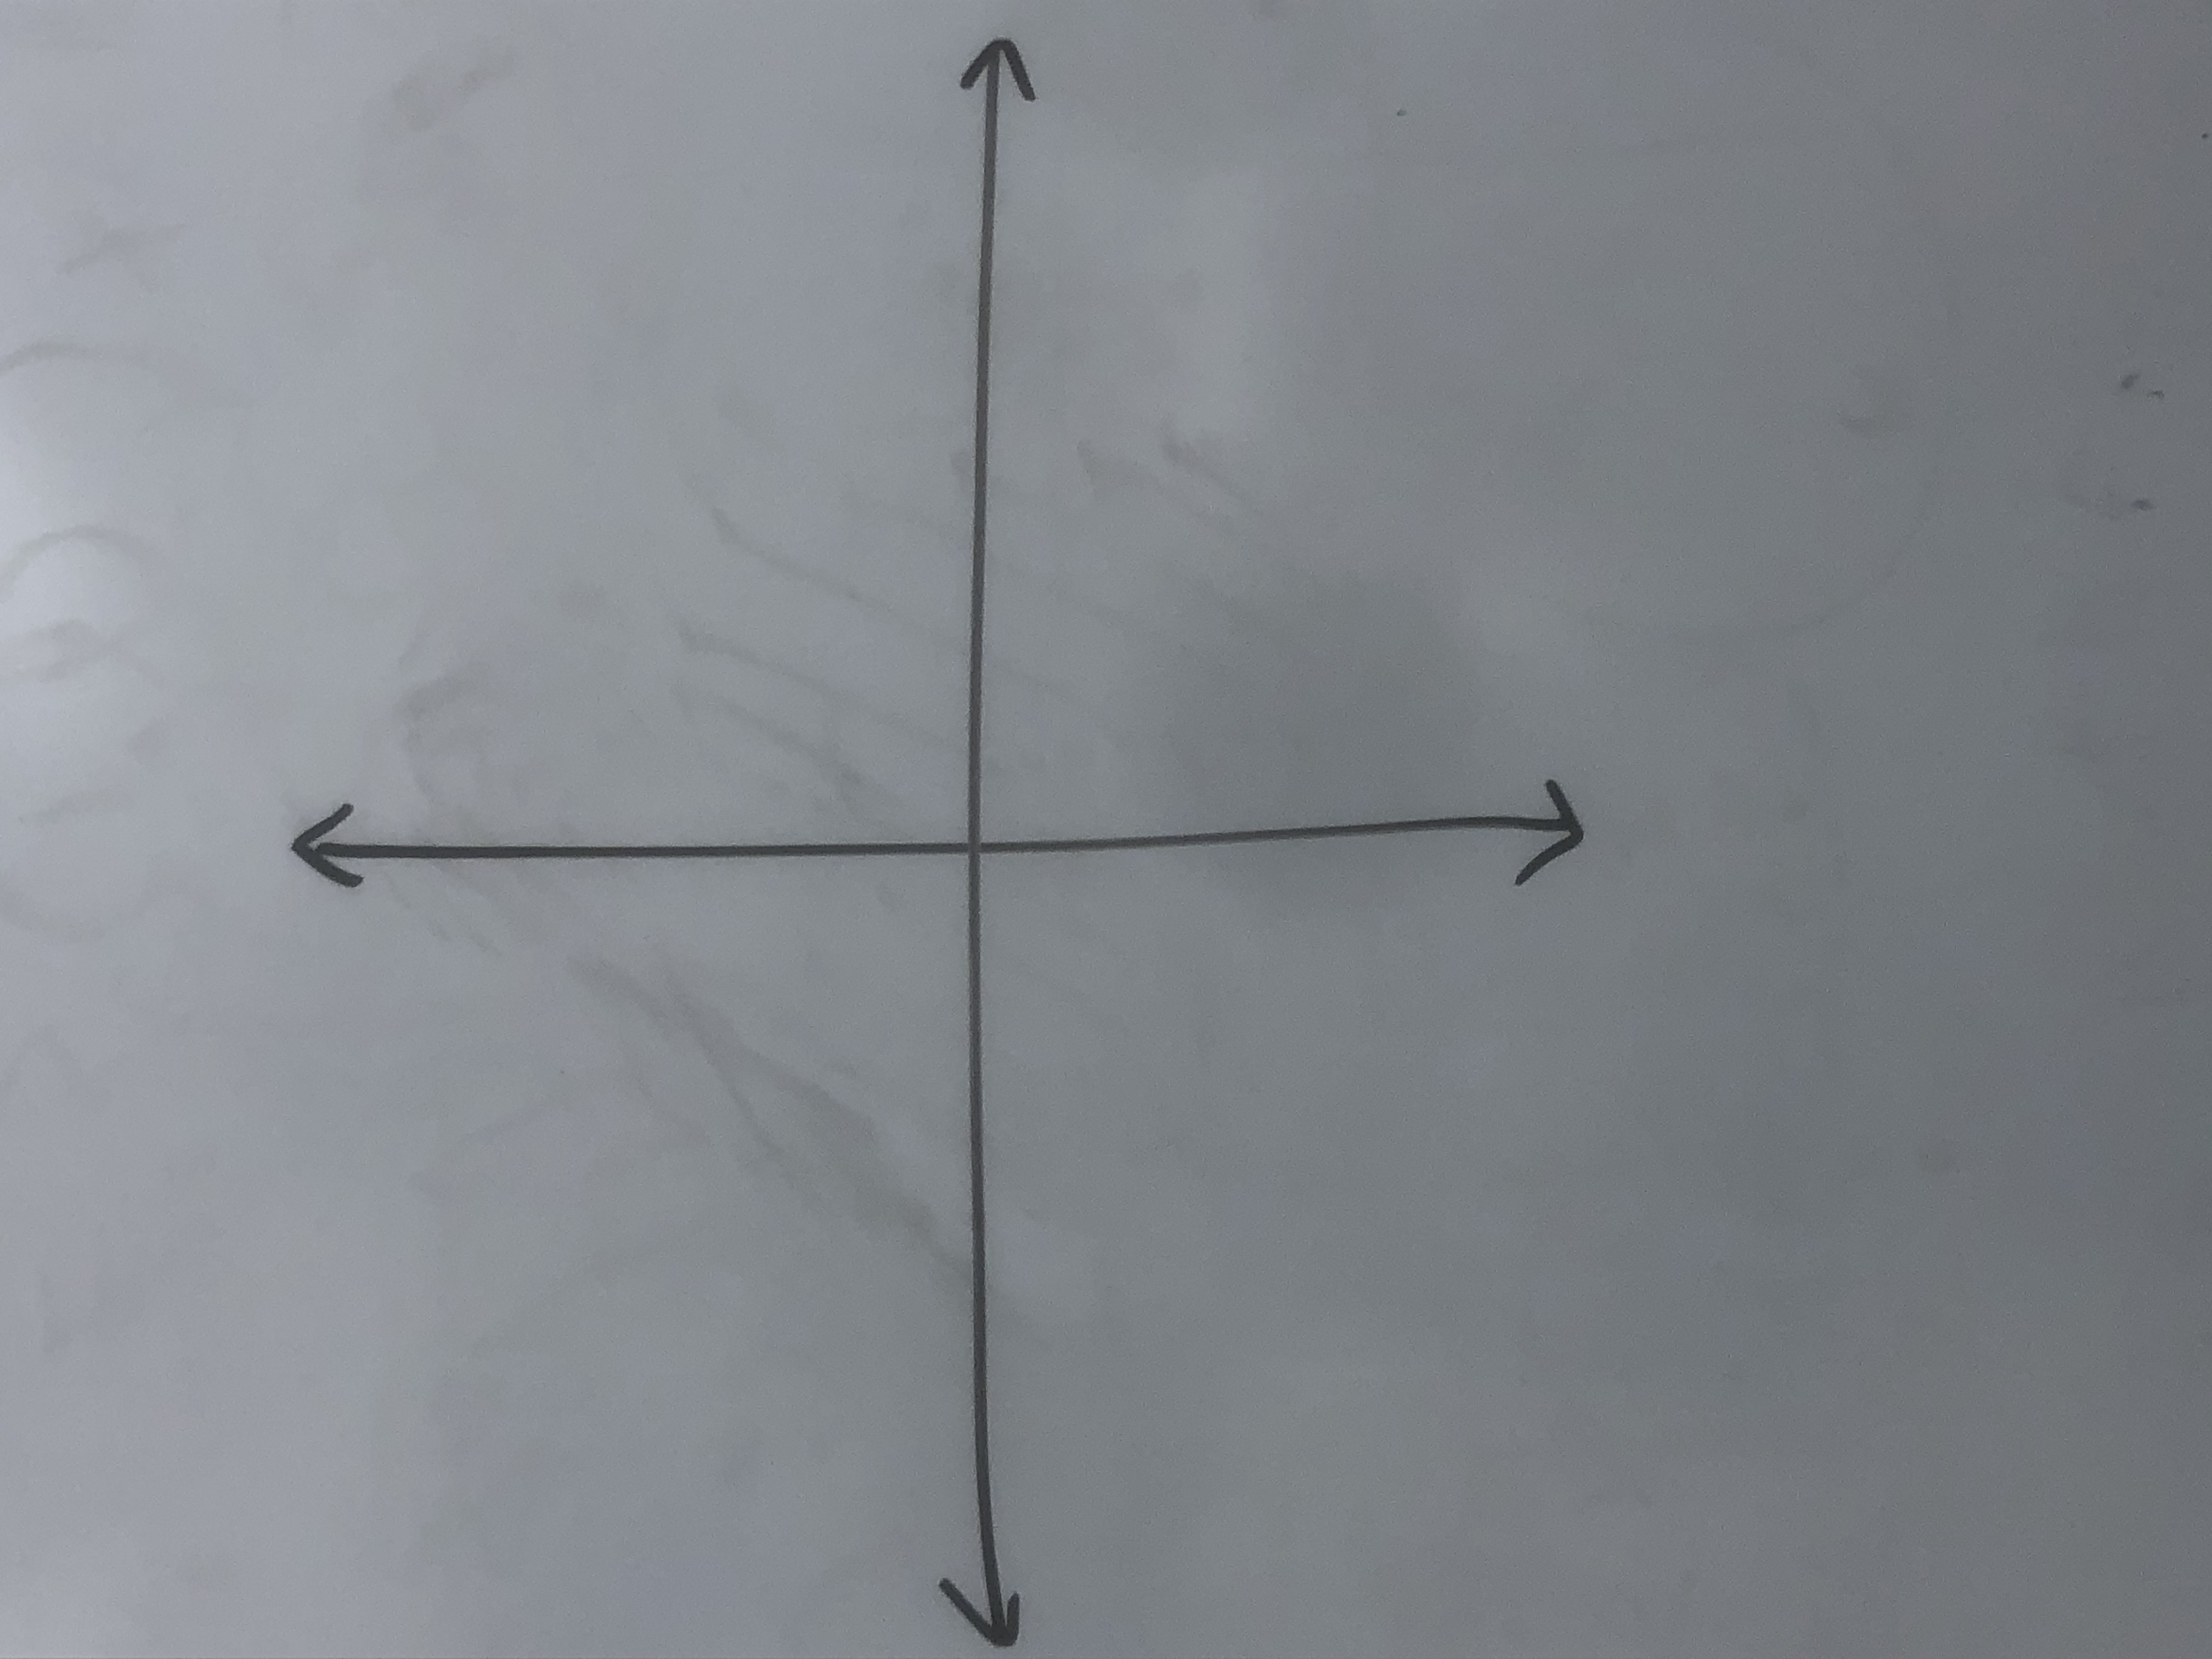
\includegraphics[scale=.05]{IMG-0797.jpg}
\end{center}

\begin{center}
A basis element for the product topology on $\R^2$:

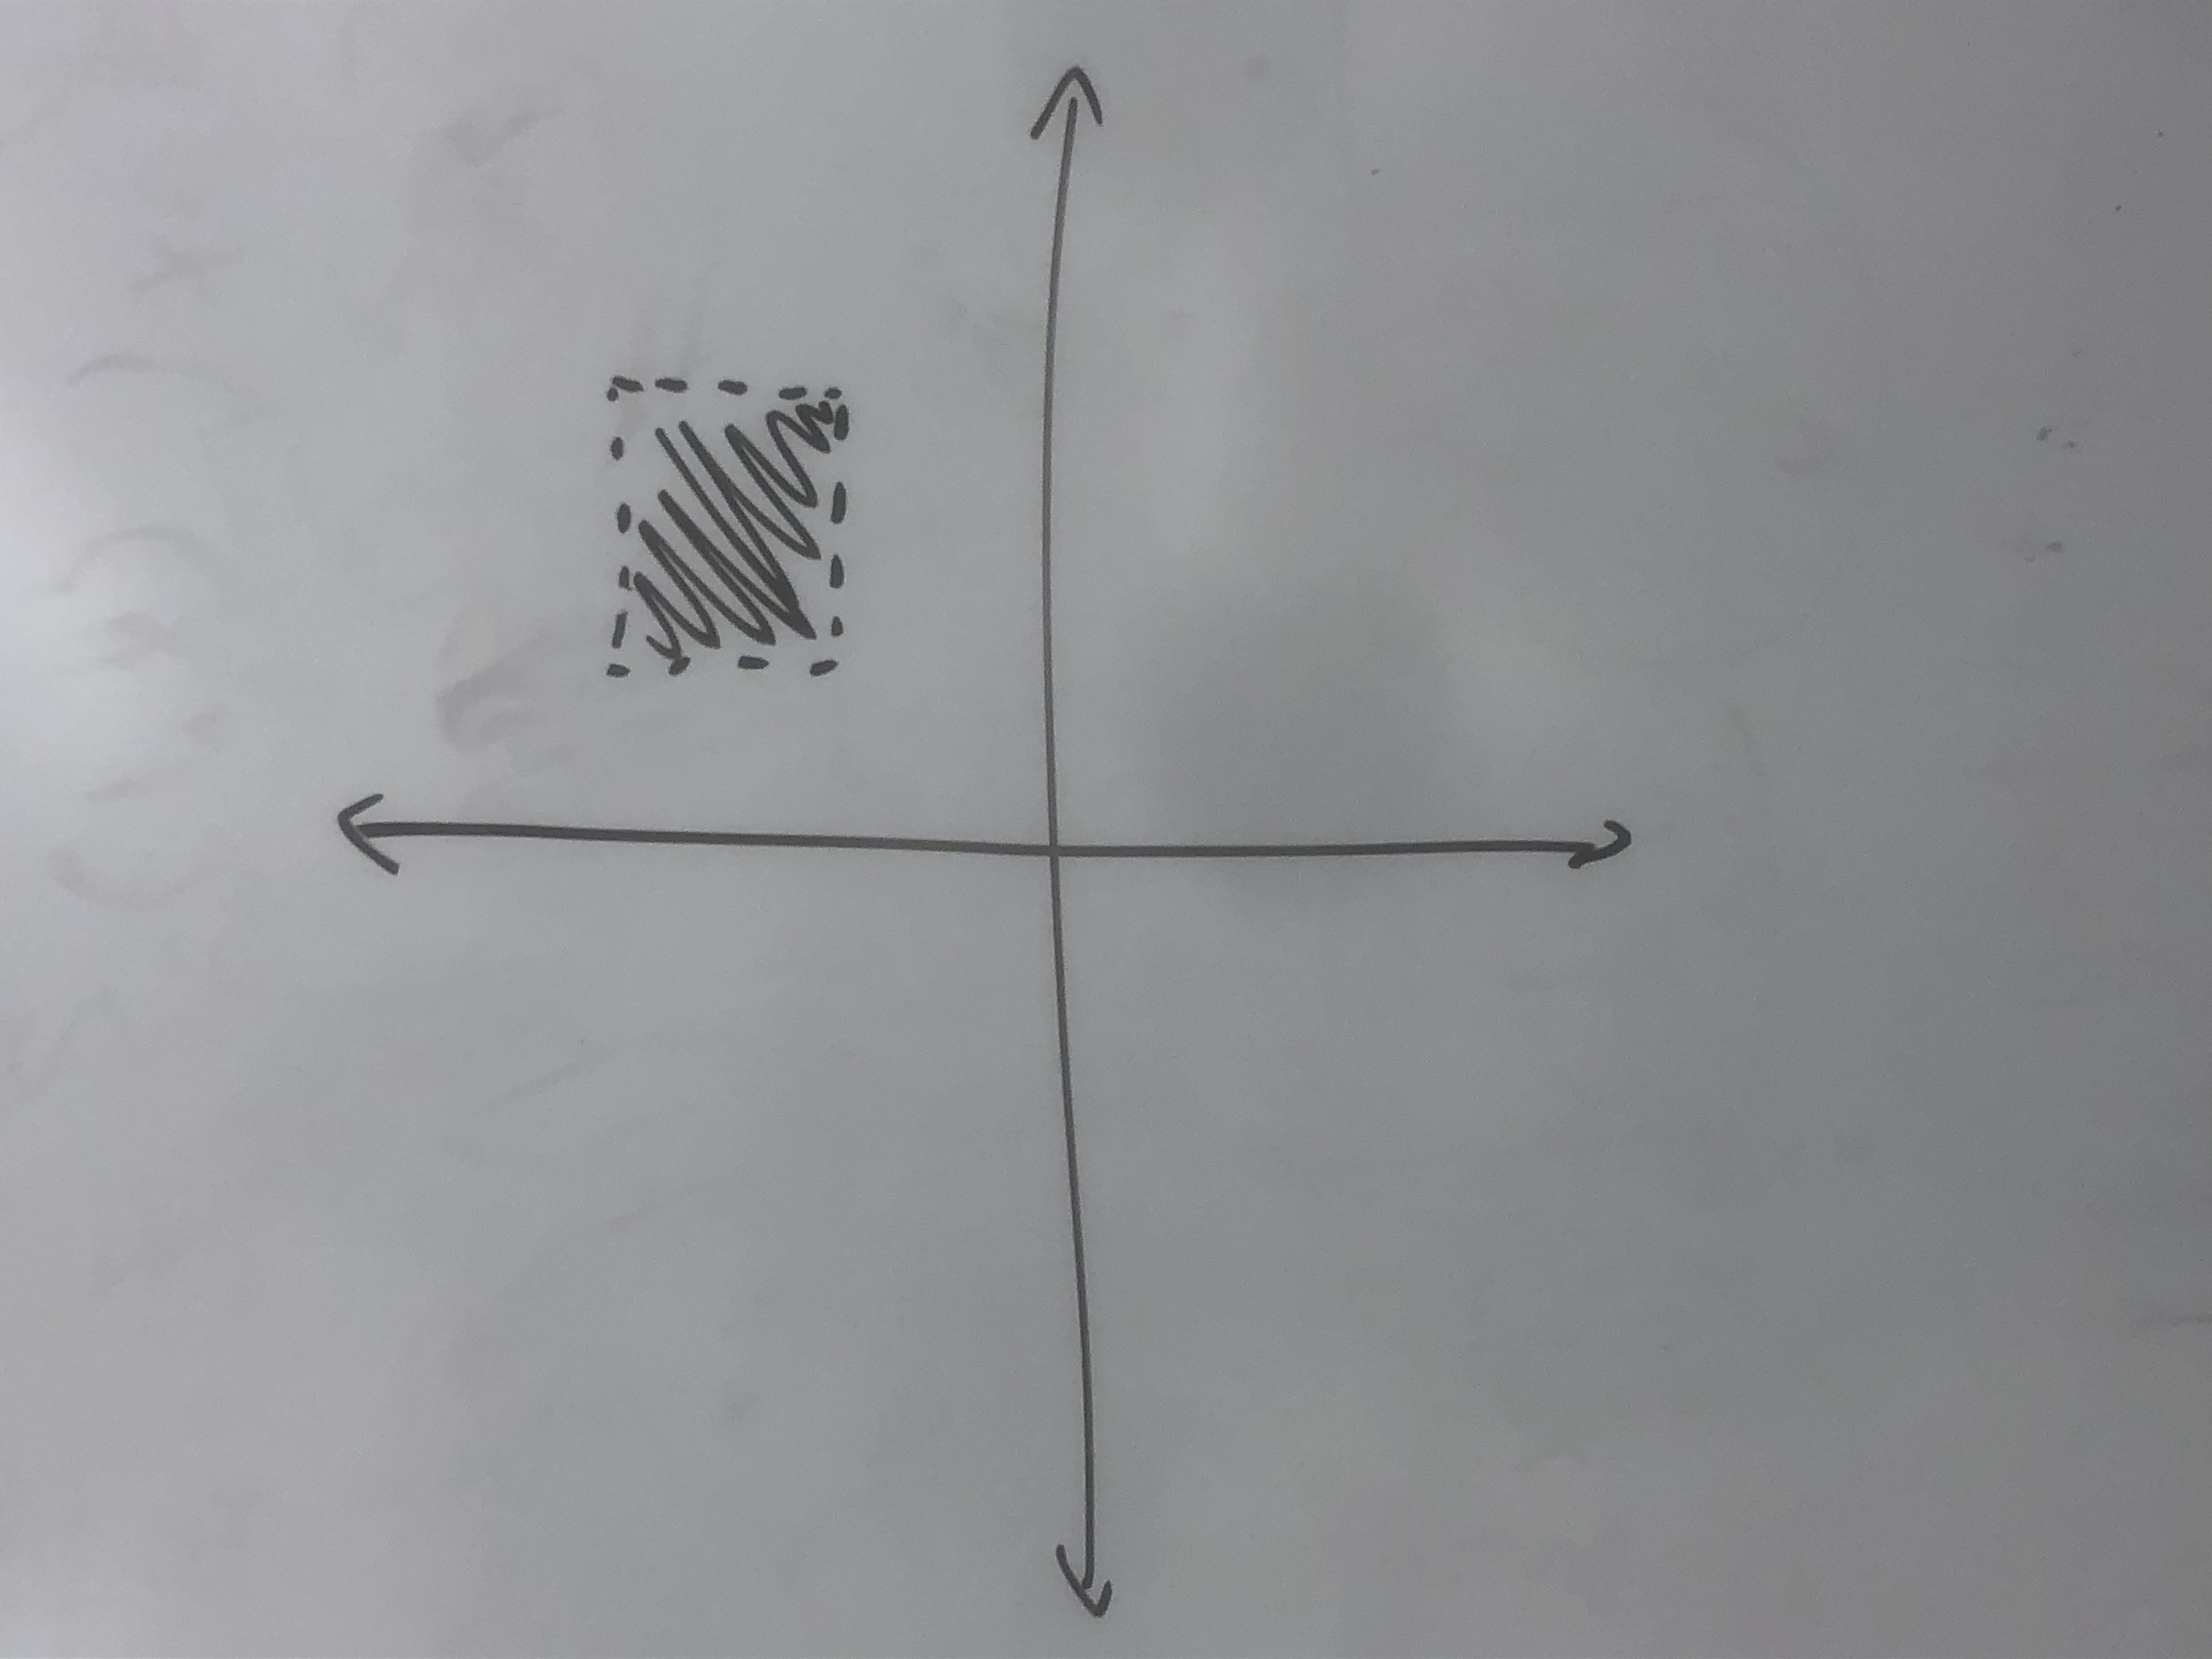
\includegraphics[scale=.05]{IMG-0795.jpg}
\end{center}

\begin{center}
A general open set in the product topology on $\R^2$:

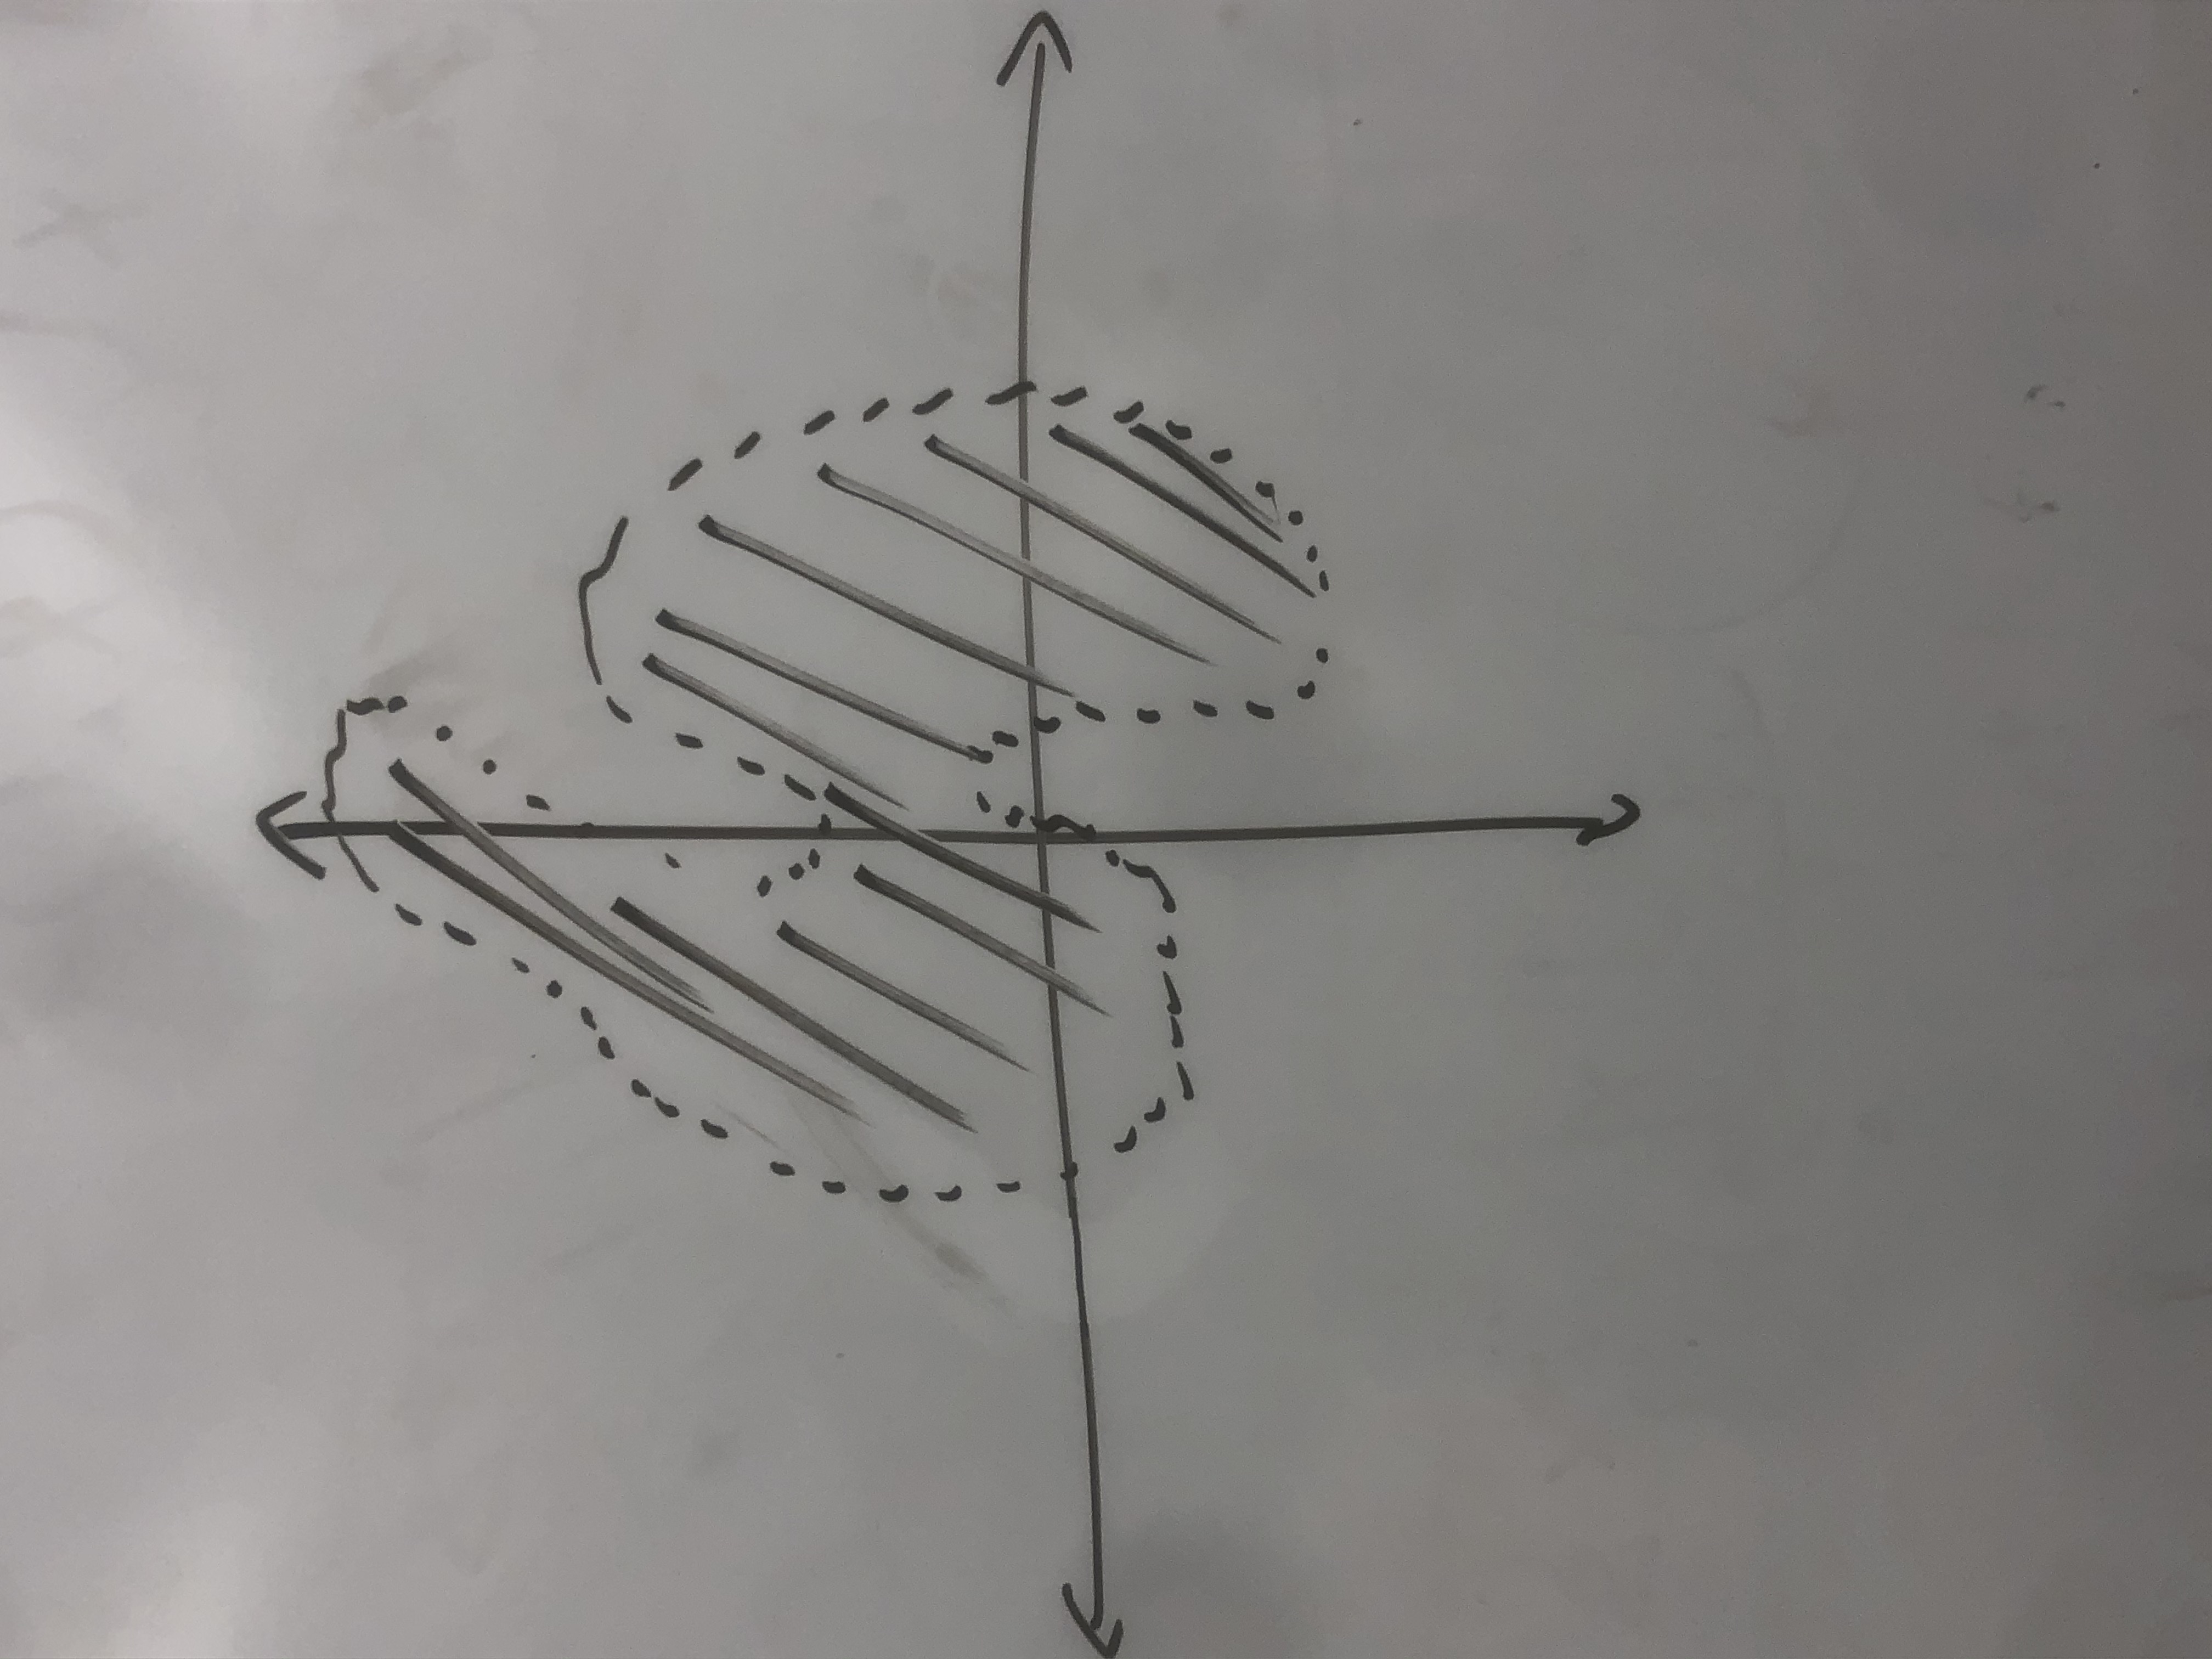
\includegraphics[scale=.05]{IMG-0796.jpg}
\end{center}

\newpage\noindent{\bf 3.}
\begin{proof}
    Let $(X, \tau)$ and $(Y, \tau')$ be topological spaces and assume that $X$ has the discrete topology denoted by $\tau$.
    Let $V$ be an open set in the product topology on $X \times Y$.
    For each $x \in X$, define $U_x$ to be $\{y \mid (x,y) \in V\}$.
    Note that by the definition of the product topology, $U_x \in \tau'$.
    Then,
    \begin{align*}
        \bigcup_{x \in X}\{x\} \times U_x &= \bigcup_{x \in X}\{x\} \times \{y \mid (x,y) \in V\} \\
                                          &= V.
    \end{align*}
    Thus, the open sets in the product topology on $X \times Y$ are exactly those subsets of $X \times Y$ of the form $\bigcup\limits_{x \in X} x \times U_x$.
\end{proof}

\newpage\noindent{\bf 4.}
\begin{proof}
    $\Z$ satisfies the condition.
    Let $a \in \Z$.
    Then, $(a-1,a+1)$ is open in the order topology on $\Z$.
    Thus, each singleton in $\Z$ is open in the order topology on $\Z$.
    Let $B \subseteq \Z$.
    Then, $B = \bigcup\limits_{b \in B} \{b\}$.
    Thus, $B$ is open in the order topology on $\Z$.
    Thus, the order topology on $\Z$ is the discrete topology on $\Z$.
\end{proof}
\end{document}